\section{Design Patterns}
Nach dem Architekten Christopher Alexander lässt sich ein Design Pattern folgendermaßen beschreiben:

"Each pattern describes a problem which occurs over and over again in our environment, and then describes the core of the solution to that problem, in such a way that you can use this solution a million times over, without ever doing it the same way twice."

Obwohl diese Aussage auf Gebäude bezogen war, lässt sie sich ebenso gut auch Softwarearchitekturen anwenden. Auch in der Planung großer Softwaresysteme treten häufig dieselben abstrakten Probleme auf, welche sich mit einer Menge von Design Patterns lösen lassen, welche die Beziehungen und Interaktionen von Objekten spezifizieren.

Ein Design Pattern besteht dabei immer aus vier Elementen, seinem Namen, einer Problembeschreibung, einer Lösung und den sich ergebenden Konsequenzen. Die Problembeschreibung gibt dabei an, in welchen Fällen ein Pattern sich anwenden lässt, während die Lösung die Beziehungen und Verantwortlichkeiten der beteiligten Objekte beschreibt. Sie geht dabei nicht auf individuelle Anwendungsfälle ein, sondern stellt lediglich eine abstrakte Herangehensweise an das Problem bereit. Jedes Pattern bringt Vor- und Nachteile mit sich und geht Kompromisse zwischen verschiedenen Qualitätsaspekten ein. Die Konsequenzen beleuchten diese  und helfen bei der Argumentation für oder gegen eine konkrete Designentscheidung.

Im Folgenden werden die abstrakten Design Patterns beschrieben, welche in der Architekturdiskussion eine Rolle spielen werden.

\subsection{Strategy Pattern}

\subsubsection*{Problembeschreibung}

Es kann vorkommen, dass mehrere Varianten eines Algorithmus benötigt werden, welche alle eine einheitliche Schnittstelle bereitstellen. Je nach Kontext wird ein anderer Algorithmus benötigt. Die Algorithmen sollen dynamisch austauschbar sein, um deren flexiblen Einsatz zu ermöglichen und eine lose Kopplung zu gewährleisten. Eine Implementierung der Algorithmen-Varianten innerhalb der ausführenden Klasse, würde deren Komplexität deutlich erhöhen. Außerdem soll die Möglichkeit bestehen, in Zukunft weitere Algorithmen hinzuzufügen. Das \emph{Strategy Pattern} kann die Übersichtlichkeit verbessern, wenn viele ähnliche Klassen existieren, die sich lediglich in ihrem Verhalten unterscheiden. Weiterhin sollen Implementierungsdetails und Algorithmus-spezifische Daten vom Kontext abgekapselt werden. \cite{gamma_design_1995}

\subsubsection*{Lösung}

Wie in \autoref{fig:strategy-class} abgebildet, besitzt der Kontext (\code{Context}), welcher einen Algorithmus verwenden soll, eine Referenz auf eine Strategie (\code{Strategy}). Die konkrete Strategie (\code{ConcreteStrategy}) wurde dem Kontext zuvor durch den Anwender (\code{Client})\footnote{Der Anwender (\code{Client}) ist in der Regel eine weitere Klasse, welche den beschriebenen Mechanismus verwendet. Es handelt sich in aller Regel nicht um einen Menschen.\label{ftn:client}} mithilfe von \code{setStrategy} zugewiesen. Die konkrete Strategie realisiert die \code{Strategy}-Schnittstelle, sodass Kontext und konkrete Strategie lediglich lose gekoppelt sind. Jede Strategie stellt die Methode \code{execute} bereit, um den gekapselten Algorithmus auszuführen.

\begin{figure}[!ht]
	\centering
	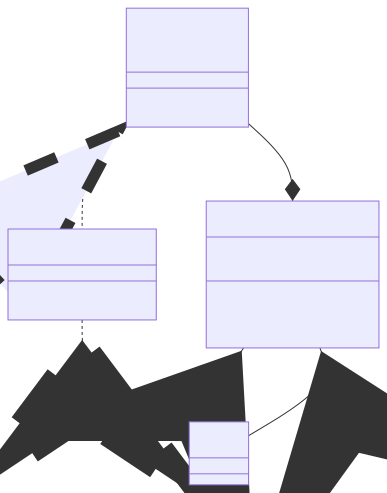
\includegraphics[width=0.75\linewidth]{images/patterns/strategy-class.pdf}
	\caption{Klassendiagramm des \emph{Strategy Patterns}. Der \code{Context} kann durch Nutzung der abstrakten \code{Strategy}-Schnittstelle eine Menge verschiedener Algorithmen nutzen, welche in konkreten Strategien implementiert sind. \cite{skobeleva_strategy_2023}}
	\label{fig:strategy-class}
\end{figure}

\autoref{fig:strategy-seq} zeigt die typische Verwendung des \emph{Strategy Patterns}. Der Kontext wird initialisiert, indem ihm vom Anwender eine konkrete Strategie zugewiesen wird (3), welche zuvor vom Anwender erzeugt wurde (1). Der Anwender kann von nun an den Kontext dazu veranlassen, eine Aktion durchzuführen, welche die Verwendung des in der hinterlegten Strategie vorhandenen Algorithmus nach sich zieht (5). Der Kontext kann den Algorithmus ausführen (6), ohne Wissen über die konkrete Strategie zu benötigen.

\begin{figure}[!ht]
	\centering
	\includegraphics[width=0.75\linewidth]{images/patterns/strategy-seq.pdf}
	\caption{Sequenzdiagramm des \emph{Strategy Patterns}. Eine konkrete Strategie wird erzeugt und dem \code{Kontext} übergeben. Dieser kann nun den in der Strategie implemenierten Algorithmus nutzen. \cite{skobeleva_strategy_2023}}
	\label{fig:strategy-seq}
\end{figure}

\subsubsection*{Konsequenzen}
Das \emph{Strategy Pattern} ermöglicht es, durch die Verwendung von Vererbung eine Hierarchie von Algorithmen aufzubauen. Das kann hilfreich sein, wenn mehrere Algorithmen sich Teile ihrer Implementierung teilen. Das Muster extrahiert die Algorithmen-Implementierung aus dessen Kontext und verhindert damit die sonst notwendige Bildung von Subklassen des Kontextes. Die Auswahl des auszuführenden Algorithmus wird über Aggregation gesteuert. Damit entfällt die Notwendigkeit von bedingten Sprüngen. Weiterhin können dank des \emph{Strategy Patterns} auch mehrere Algorithmen bereitgestellt werden, deren Verhalten identisch ist und sich beispielsweise nur in der Performance unterscheiden. So kann je nach Laufzeitumgebung eine Entscheidung für eine bessere Laufzeit oder einen effizienteren Umgang mit Speicherressourcen getroffen werden.

Nachteile des \emph{Strategy Patterns} sind zum einen ein erhöhter Mehraufwand für Kommunikation. Unter Umständen benötigt ein Algorithmus nicht die gesamte Schnittstelle, um zu funktionieren. Da der Kontext allerdings nur die abstrakte Schnittstelle der Strategie kennt, muss er stets die gesamte Schnittstelle bedienen. Das bedeutet unnötige Aufrufe von Methoden oder unnötige Übergabe von Parametern. Weiterhin erhöht dieses Muster die Gesamtzahl an Objekten und damit die Komplexität zur Laufzeit. \cite{gamma_design_1995}
\subsection{Template Method}

\subsubsection*{Problembeschreibung}

Es existieren ein Algorithmus, welcher aus einer Menge von Teilschritten besteht. Die einzelnen Teilschritte sollen austauschbar gehalten werden, um ein flexibles Anpassen des Algorithmus zu ermöglichen. Die Reihenfolge der Teilschritte ist hingegen festgelegt. 

\subsubsection*{Lösung}

\begin{figure}[!hb]
	\centering
	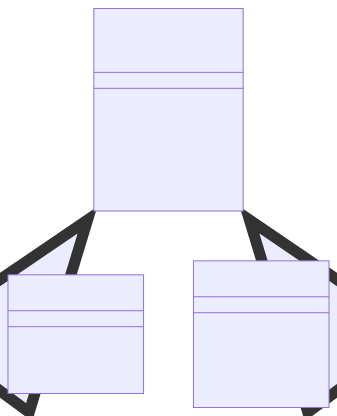
\includegraphics[width=0.75\linewidth]{images/patterns/template-method-class.png}
	\caption{Klassendiagramm Template Method}
	\label{fig:template-method-class}
\end{figure}

Jede Klasse, welche einen Algorithmus der selben Struktur implementiert, erbt von einer abstrakten Klassen, welche die `templateMethod` implementiert. Diese gibt das Grundgerüst des Algorithmus vor und ruft darin die einzelnen Teilschritte auf. Diese sind jeweils in eigenen Methoden implementiert. Die Subklassen definieren diese Methoden zum Teil neu, wenn eine Veränderung des Verhaltens dieses Teilschrittes notwendig ist.


\lstset{language=python}
\begin{lstlisting}[caption={Quelltextunterschrift}, label=code:template-method-code]
class AbstractClass:
	def templateMethod(self):
    	if self.step1():
        	self.step2()
    	self.step3()
\end{lstlisting}


\subsubsection*{Konsequenzen}

Template Methods sind ein Mechanismus, welcher die Wiederverwendung von Code ermöglicht und kann somit der Codeduplikation entgegen wirken. Anstatt Abwandlungen von Algorithmen von Grund auf neu zu implementieren, ist es möglich, sie aus bestehenden Komponenten zusammenzusetzen und je nach Bedarf neuen Code hinzuzufügen. Das Muster der Template-Method weist eine umgekehrte Kontrollstruktur auf. Anstatt dass eine Klasse Methoden ihrer Superklasse aufruft, delegiert die Template-Method die Verantwortlichkeit für die einzelnen Teile des Algorithmus an sie Subklassen.

Bei der Verwendung der Template-Method ist jedoch zu beachten, wie die einzelnen Methoden zu verwenden sind. Diese lassen sich grob in zwei Arten einteilen, Die "Hook"-Methoden und die abstrakten Methoden. Während die "Hook"-Methoden eine Standard-Implementierung in der abstrakten Basisklasse bereitstellen, ist dies bei den abstrakten Methoden nicht der Fall. Entsprechend müssen die abstrakten Methoden zwingend von einer konkreten Subklasse implementiert werden. Bei den "Hook"-Methoden ist das optional. 

Die Template-Method synergiert mit dem Strategy-Pattern. Einzelne Schritte eine Algorithmus können in einer Strategie-Klasse implementiert sein.
\subsection{Observer Pattern}


\subsubsection*{Problembeschreibung}

Häufig müssen verschiedene Komponenten eines Systems synchron gehalten werden. Gleichzeitig soll aber auch eine enge Kopplung dieser Komponenten vermieden werden. Es wird eine $1$:$n$-Beziehung zwischen den Objekten benötigt. Wenn ein Objekt seinen Zustand ändert, so sollen alle abhängigen Objekte benachrichtigt werden, sodass auch sie ihren Zustand aktualisieren können. Ein naiver Lösungsansatz wäre, jedem abhängigen Objekt eine Referenz auf das Objekt zu geben, von welchem es abhängt. Die Objekte könnten dann in regelmäßigen Abständen prüfen, ob eine Zustandsänderung stattgefunden hat. Dieser Ansatz weist jedoch nicht nur eine hohe Kopplung auf, er ist auch wenig performant. Auch wenn keine Zustandsänderung stattgefunden hat, wird auf diese geprüft. Der Aufwand für diese Prüfung steigt dabei linear mit der Anzahl der beteiligten Objekte.

Das Observer-Pattern kann Anwendung finden, wenn es zwei voneinander getrennte Konzepte gibt und eines von dem anderen abhängig ist. Die Abhängigkeit kann modelliert werden, ohne die Objekte zu koppeln. Weiterhin ist es möglich, die Anzahl der abhängigen Objekte variablen zu halten.  

\subsubsection*{Lösung}

Das Observer-Pattern besteht aus einem Publisher und mehreren Subscribern. Die Subscriber implementieren das Subscriber-Interface, welches eine Methode `update`  zur Aktualisierung des Zustandes bereitstellt. Der Publisher hält eine Liste von Referenzen auf Subscriber und verfügt über die Methoden `subscribe` und `unsubscribe`, welche es ermöglichen, der Liste Subscriber hinzuzufügen, oder sie zu entfernen. 

\begin{figure}[!hb]
	\centering
	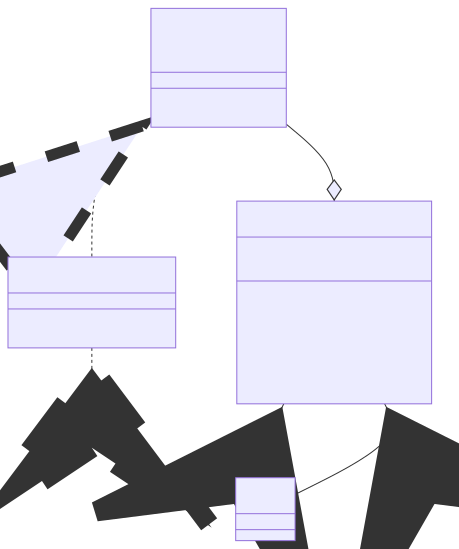
\includegraphics[width=0.75\linewidth]{images/patterns/observer-class.png}
	\caption{Klassendiagramm Observer}
	\label{fig:observer-class}
\end{figure}

Der Client kann den Zustand des Publishers durch Senden von `updateSate` verändern (1). Der Publisher sendet sich draufhin selbst `notify` (2) und beginnt über seine Liste von Subscribern zu iterieren. Jedem Subscriber sendet er dann `update` (3, 5) und übergibt den notwendigen Kontext, sodass der Subscriber seinen Zustand entsprechend aktualisieren kann. 

\begin{figure}[!hb]
	\centering
	\includegraphics[width=0.75\linewidth]{images/patterns/observer-seq.png}
	\caption{Sequenzdiagramm Observer}
	\label{fig:observer-seq}
\end{figure}

Der folgende Code veranschaulicht die Benachrichtigung aller Subscriber. In `notify` wird an jeden im Publisher referenzierten Subscriber `update` gesendet. Dabei wird der Kontext des Publishers an jeden Subscriber übergeben.

\lstset{language=python}
\begin{lstlisting}[caption={Quelltextunterschrift}, label=code:template-method-code]
class Publisher
	def notify(self):
        for subscriber in self.subscribers:
            subscriber.update(self.context)
\end{lstlisting}


\subsubsection*{Konsequenzen}

Template Methods sind ein Mechanismus, welcher die Wiederverwendung von Code ermöglicht und kann somit der Codeduplikation entgegen wirken. Anstatt Das Observer-Pattern bietet eine Reihe von Vorteilen. Durch Separation von Publisher und Subscriber und durch die Abstraktion des Subscriber-Interfaces wird eine lose Kopplung der beiden erreicht. Diese lose Kopplung ermöglicht es, sowohl den Publisher, als auch die Subscriber beliebig auszutauschen. Weiterhin können sich der Publisher und die Subscriber auf unterschiedlichen Abstraktionsniveaus befinden. Ein Publisher auf einem niedrigen Level kann einen Subscriber auf einem hohen Level benachrichtigen. Wären Subscriber und Publisher nicht getrennt, so wäre dafür ein Abstraktionshierarchie-übergreifendes Objekt notwendig, welches die Trennung der Abstraktionsschichten beeinträchtigen würde. Ein weiterer Vorteil ist die dynamische Anzahl der Subscriber, mit denen ein Publisher interagieren kann. So kann der Client über den Publisher eine beliebige Zahl an Subscribern erreichen.

Ein Nachteil des Observer-Patterns ist, dass der Publisher stets alle seine Subscriber benachrichtigt. Es kann vorkommen, dass nur eine Teilmenge der Subscriber die Benachrichtigung benötigt, was in unnötigen Methodenaufrufen resultiert.
\subsection{Mediator Pattern}


\subsubsection*{Problembeschreibung}

Große Softwareprojekte bestehen meist aus einer einer enormen Anzahl an Klassen bzw. Objekten, welche miteinander interagieren. Ziel ist es stets, die Kopplung zwischen diesen Komponenten so gering wie möglich zu halten. Komplexe Interaktionsmuster zwischen diesen Objekten lassen sich nicht immer verhindern, das sie die inhärente Komplexität des modellierten Problems wiederspiegeln. In diesem Fall ist eine Lösung notwending, die diese Komplexität kapselt. Das Mediator-Pattern ist in der Lage, solche Fälle von komplexer Interaktion zu vereinfachen.

\subsubsection*{Lösung}

Der konkrete Mediator implementiert das Mediator-Interface, welches eine Methode `notify` bereitstellt, um Benachrichtigungen der einzelnen Komponenten entgegenzunehmen. Jede Komponente besitzt eine Referenz auf den Mediator, um `notify`an ihn senden zu können. Dabei übergibt die Komponente sich selbst, um dem Mediator den Kontext der Benachrichtigung bereitzustellen. In Abhängigkeit des übergebenen Senders und dessen Zustand, führt der Mediator eine (komplexe) Logik aus, welche vollständig innerhalb des Mediators gekapselt ist. Der Mediator hält ebenso Referenzen auf alle Komponenten, die er zu beeinflussen in der Lage sein soll. Die gekapselte Logik kann somit die Interfaces der Komponenten verwenden, um diese zu beeinflussen. Dadurch findet eine indirekte Beeinflussung von Komponenten durch andere Komponenten über den Mediator statt.  

\begin{figure}[!hb]
	\centering
	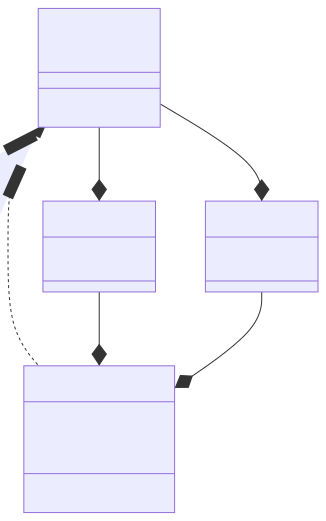
\includegraphics[width=0.75\linewidth]{images/patterns/mediator-class.png}
	\caption{Klassendiagramm Mediator Pattern}
	\label{fig:mediator-class}
\end{figure}

\subsubsection*{Konsequenzen}

Der Mediator kapselt Verhalten, welches ansonsten über mehrere Klassen verteilt wäre. Soll dieses Verhalten spezialisiert werden, so ist nur eine Spezialisierung des Mediators notwendig. Weiterhin verhindert der Mediator eine starke Kopplung der Komponenten. Komponenten- und Mediator-Klassen können bei kompatiblen Interfaces beliebig ausgetauscht werden. Der Mediator vereinfacht außerdem die Multiplizitäten von Objektinteraktionen. Er wandelt $m$:$n$- Beziehungen zwischen Objekten in $1$:$n$-Beziehungen zwischen den Objekten und dem Mediator um. 

Der Mediator bündelt Kontrolle an einem einzigen Punkt. Dies kann zur Übersichtlichkeit beitragen, kann dieser jedoch bei ausreichend komplexer Logik entgegenwirken. Das kann dem Mediator eine monolithische Struktur geben, deren Verhinderung seine eigentliche Aufgabe ist. 

Sind die Abhängigkeiten zwischen den Komponenten zu Komplex, so kann das Observer-Pattern zur Kommunikation zwischen den Komponenten und dem Mediator verwendet werden. Dadurch lassen sich die Abhängigkeiten außerdem flexibler gestalten, sie können also zur Laufzeit einfacher geändert werden.
\subsection{\emph{Visitor Pattern} und \emph{Double Dispatch}}


\subsubsection*{Problembeschreibung}

Gelegentlich muss eine Operation auf einer Menge von Objekten durchgeführt, die alle Teil einer Objekthiearchie aber unterschiedlich sind. Diese Objekte besitzen daher unter Umständen voneinander abweichende Schnittstellen. Das \emph{Visitor Pattern} erlaubt es, solche Operationen außerhalb der Objekte und für alle betroffenen Objekte innerhalb einer separaten Klasse zu definieren. \cite{gamma_design_1995}

\subsubsection*{Lösung}

Der konkrete \emph{Visitor}\footnote{Die deutsche Übersetzung ''Besucher'' ist in diesem Kontext eher unüblich.} (\code{ConcreteVisitor}) realisiert die \emph{Visitor}-Schnittstelle (\code{Visitor}), welche die Methode \code{visit} bereitstellt, wie in \autoref{fig:visitor-class} zu erkennen ist. Diese erlaubt es dem \emph{Visitor}, ein Element (\code{Element}) zu ''besuchen'' und auf ihm eine Operation durchzuführen. Die Elemente ''akzeptieren'' den ''Besuch'' des \emph{Visitors} mit Hilfe der Methode \code{accept}, welche als Argument den besuchenden \emph{Visitor} erhält.

\begin{figure}[!ht]
	\centering
	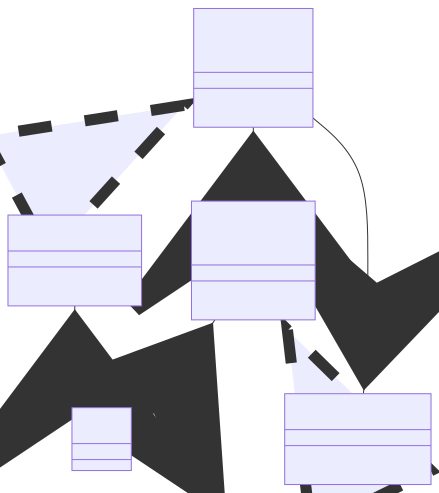
\includegraphics[width=0.75\linewidth]{images/patterns/visitor-class.pdf}
	\caption{Klassendiagramm des \emph{Visitor Patterns}. Der \code{Visitor} kapselt eine Operation auf einer Menge von Elementen in seinen \code{visit}-Methoden. Die Elemente werden von dem \code{Visitor} ''besucht'' und rufen die zu ihrem Typ korrespondierende Methode auf dem Visitor auf. \cite{skobeleva_visitor_2023}}
	\label{fig:visitor-class}
\end{figure}

\autoref{fig:visitor-seq} zeigt das Verhalten des \emph{Visitor Patterns}. Der Anwender\footref{ftn:client} trägt dem \emph{Visitor} auf, eine Operation auf einem Element oder einer Menge von Elementen durchzuführen (1). Der \emph{Visitor} sendet daraufhin \code{visit} an alle Elemente, auf die er eine Referenz hält (2). Jedes Element ruft daraufhin eine \code{accept}-Methode auf dem \emph{Visitor} auf (3). Zu beachten ist hierbei, dass es für jede Element-Klasse eine eigene Methode im \emph{Visitor} gibt. Dies kann realisiert werden durch das Bereitstellen von Methoden mit unterschiedlichen, zu den aufrufenden Klassen korrespondierenden Namen oder durch Multimethoden. Multimethoden sind Methoden, welche je nach Typ der übergebenen Argumente unterschiedliche Implementierungen ausführen. Somit kann der \emph{Visitor} nach Erhalt von \code{accept} die zum Typ des sendenden Elements passende Operation ausführen. Dieser Mechanismus nennt sich \emph{Double Dispatch}.

\begin{figure}[!ht]
	\centering
	\includegraphics[width=0.75\linewidth]{images/patterns/visitor-seq.pdf}
	\caption{Sequenzdiagramm des \emph{Visitor Patterns}. Das Entwurfsmuster nutzt einen \emph{Double Dispatch}, um die Ausführung der korrekten Methode im \code{Visitor}-Objekt zu gewährleisten. Dazu ruft der Visitor auf dem Element die Methode \code{accept} auf (2). Diese ruft dann die zum Element passende \code{visit}-Methode auf (3). \cite{skobeleva_visitor_2023}}
	\label{fig:visitor-seq}
\end{figure}

\subsubsection*{Konsequenzen}
Durch die Kapselung der Operation in einem \emph{Visitor}, ist es sehr einfach, neue Operationen hinzuzufügen. Es bedarf dazu lediglich eines weiteren \emph{Visitors}. Außerdem kapselt ein \emph{Visitor} die Menge an Operationen auf den Elementen. Zusammengehörige Operationen werden in einer Klasse gesammelt. Nicht zueinander gehörende Operationen befinden sich in unterschiedlichen \emph{Visitors}. Ein weiterer Vorteil eines \emph{Visitors} ist dessen Fähigkeit, während des ''Besuchens'' mehrerer Elemente Informationen über diese zu akkumulieren und im Anschluss gebündelt zu repräsentieren.

Der \emph{Visitor}weist jedoch auch Nachteile auf. Zum einen ist es schwer, weitere konkrete Element-Klassen zu einem System hinzuzufügen, welches bereits eine Reihe an \emph{Visitors} besitzt. Da ein \emph{Visitor} für jeden Typ von Element eine Methode bereitstellen muss, kann ein weiteres Element einen erhöhten Implementierungsaufwand bedeuten. Das \emph{Visitor Pattern} sollte daher nur verwendet werden, wenn entweder die Menge an Elementklassen abgeschlossen oder die Menge an \emph{Visitor}-Klassen übersichtlich ist. Weiterhin müssen die Elemente dem \emph{Visitor} eine Schnittstelle bereitstellen, welche es dem \emph{Visitor} ermöglicht, seine Operation ausführen zu können. Dies kann dazu führen, dass das Element einen großen Teil seines internen Zustands preisgeben muss, welcher bei nicht-Verwendung dieses Musters gekapselt geblieben wäre. \cite{gamma_design_1995}
\subsection{Factory Method}

\subsubsection*{Problembeschreibung}

Es wird ein Interface benötigt, um eine Reihe von konkreten Produkten erzeugen zu können. Jedes konkrete Produkt hat jedoch andere Anforderungen an seine eigene Erzeugung. Eine Factory-Method kann eingesetzt werden, wenn eine Klasse kein Wissen darüber besitzt oder besitzen soll, welches konkrete Produkt sie zu erzeugen hat oder eine Klasse die Verantwortlichkeit über diese Entscheidung ihren Subklassen überlassen möchte.

\subsubsection*{Lösung}

Es existiert ein eine abstrakte `Creator`-Klasse, welche ein Interface bereitstellt, um Produkte zu erzeugen. Die Details der Erzeugung dieser Produkte sind in den konkreten Subklassen von `Creator` implementiert. Jeder konkrete `Creator` kann somit einen Typ von konkretem Produkt erschaffen.

\begin{figure}[!hb]
	\centering
	\includegraphics[width=0.75\linewidth]{images/patterns/factory-method-class.png}
	\caption{Klassendiagramm Factory Method}
	\label{fig:factory-method-class}
\end{figure}

\subsubsection*{Konsequenzen}
Ein Objekt über eine Factory-Method zu erzeugen ist flexibler, als das Objekt direkt über den Konstruktor der Klasse zu instanziieren. Die erzeugende Klasse braucht nur das Interface des abstrakten `Creator` zu kennen und ist somit in der Lage beliebige konkrete Produkte über  deren korrespondierende konkrete `Creator` zu erzeugen. Hierbei fällt auf, dass die `Creator`-Klassenhierarchie die Produkt-Klassenhierarchie spiegelt. Für jeden Produkttyp existiert also auch eine `Creator`-Klasse. Daraus kann sich jedoch auch ein Nachteil ergeben. Zur Nutzung eines Produktes müssen nun stets zwei Subklassen definiert und zur Laufzeit ein weiteres Objekt erstellt werden. Das erhöht die Komplexität. 

